\documentclass[10pt,xcolor=dvipsnames]{beamer}
\usepackage[english]{babel}
\usepackage{amsmath}
\usepackage{amstext}
\usepackage{amsthm}
\usepackage{amssymb}
\usepackage{appendix}
\usepackage{array}
\usepackage[style=authoryear-comp,backend=bibtex,uniquename=init,firstinits=true,maxcitenames=2,mincitenames=1,maxbibnames=10,isbn=false,doi=false,url=false,date=year]{biblatex}
\makeatletter
\def\blx@maxline{77}
\makeatother
\usepackage{booktabs}
\usepackage{calc}
\usepackage[small,bf,format=hang,labelsep=space]{caption}
\usepackage{color}
\usepackage{colortbl}
\usepackage{contour}
\usepackage{epsfig}
\usepackage{esvect}
\usepackage{exscale}
\usepackage{fancyvrb}
\usepackage{fnpct}
\usepackage{framed}
\usepackage{graphicx}
\usepackage{listings}
\usepackage{mathrsfs}
\usepackage[version=3]{mhchem}
\usepackage{multirow}
\usepackage{pgfgantt}
\usepackage{pstool}
\usepackage{ragged2e}
\usepackage{rotating}
\usepackage{setspace}
\usepackage{siunitx}
\usepackage{subfig}
\usepackage[normalem]{ulem}
\usepackage[listings,skins,theorems]{tcolorbox}
\usepackage{tikz}
\usepackage[absolute,overlay]{textpos}
\usepackage{wasysym}

% FOR GERMAN

% \usepackage[utf8]{inputenc}
% \usepackage[T1]{fontenc}
% \usepackage{textcomp}
% \usepackage{csquotes}

% PATHS

\graphicspath{{./}{fig/}}
% \DefineBibliographyStrings{ngerman}{andothers = {\em u\adddot a\adddot}} %\em u\adddot\addabbrvspace a\adddot

\setlength{\parindent}{0 cm}
\let\raggedright\relax
\setbeamerfont{caption}{size=\footnotesize}
\setlength{\abovecaptionskip}{5pt plus 0pt minus 0pt} % Default 10pt plus 0pt minus 0pt
\allowdisplaybreaks[4]

% SANS-SERIF

\usefonttheme[onlymath]{serif} % serif, default
\setbeamertemplate{frametitle continuation}{} % Remove frame continuation numbering

% SECTION TITLE PAGES

\setbeamertemplate{bibliography item}{\insertbiblabel}
% \AtBeginSection{\frame{\centering\Large\usebeamercolor[fg]{title}\insertsection}}
% \AtBeginSubsection{\frame{\centering\Large\usebeamercolor[fg]{title}\insertsubsection}}

% LENGTH VARIABLES

\newcommand*{\itemskip}{0.25\baselineskip}

% BIBLIOGRAPHY

\addbibresource{fluid.bib}
\addbibresource{pbe.bib}
\addbibresource{rom.bib}
\renewbibmacro{in:}{}
\renewcommand\newunitpunct{\addcomma\space}
\AdaptNoteOpt{\footcite}{\multfootcite}

% POSITIONING (for textpos)

\TPGrid{20}{20}

% BOXED ENVIRONMENTS

\renewcommand{\cite}{\parencite}
\newcommand*{\citet}{\textcite}
\newtcolorbox{mybox}[2][]{colback=white,colframe=structure,colbacktitle=white,coltitle=structure,boxrule=0.5pt,arc=0mm,adjust text={\LargeÄpgjy},adjusted title=#2,#1}
\newtcolorbox{frbox}[1][]{colback=white,colframe=structure,colbacktitle=white,coltext=black,boxrule=0.5pt,arc=0mm,halign=center,title={},#1}

% BEAMER

\definecolor{myred}{RGB}{190,30,60} % Equal to \definecolor{myred}{HTML}{BE1E3C}
\definecolor{myred}{RGB}{149,27,128} % OVGU purple, equal to 951B80
\definecolor{ovgu_purple}{RGB}{149,27,128}
\definecolor{ovgu_purple_light}{RGB}{255,255,255}
\definecolor{ovgu_purple_very_light}{RGB}{244,226,236}
\colorlet{shadecolor}{myred!5}
\setbeamercolor{structure}{fg=myred,bg=white}
\setbeamercolor{frametitle}{fg=white,bg=myred}
\newcommand{\myrule}[2]{\textcolor{myred}{\rule{#1}{#2}}}
\tcbset{highlight math style={colframe=white,colback=shadecolor,arc=0pt,boxrule=0.5pt,left=0mm,right=0mm,top=0mm,bottom=0mm}}
\newcommand*\circled[1]{\tikz[baseline=(char.base)]{\node[shape=circle,draw,inner sep=2pt] (char) {#1};}}

% LETTERS

% MATH OPERATORS

\DeclareMathOperator \diag {diag}
\DeclareMathOperator \intr {int}
\DeclareMathOperator \rank {rank}
\DeclareMathOperator \tr   {tr}
\DeclareMathOperator \Div {Div}
\DeclareMathOperator \sgn {sgn}
\DeclareMathOperator \ceil {ceil}
\DeclareMathOperator \vol {vol}
\DeclareMathOperator \symm {symm}
\DeclareMathOperator \tol {tol}

% MATH

\newcommand{\R}{\mathds{R}}
\newcommand{\C}{\mathds{C}}
\newcommand{\F}{\mathds{F}}
\newcommand{\N}{\mathds{N}}
\newcommand{\Q}{\mathds{Q}}
\newcommand{\Z}{\mathds{Z}}
%% \newcommand{\IR}{\hbox{{\rm I}\kern-.1667em\hbox{{\rm R}}}} 
%% \newcommand{\IC}{\hbox{{\rm C}\kern-.4167em\hbox{\rule[.03ex]{.12ex}{1.5ex}}\kern.3567em}} 
%% \newcommand{\IF}{\hbox{{\rm I}\kern-.1667em\hbox{{\rm F}}}} 
%% \newcommand{\IZ}{\hbox {\sf Z\kern-.32em\hbox{Z}}} 
%% \newcommand{\IQ}{\hbox{{\rm Q}\kern-.4827em\hbox{\rule[.03ex]{.12ex}{1.55ex}}}}

% Capital Roman Letters

\newcommand{\Aset}{{\mathbb A}}
\newcommand{\Bset}{{\mathbb B}}
\newcommand{\Cset}{{\mathbb C}}
\newcommand{\Dset}{{\mathbb D}}
\newcommand{\Eset}{{\mathbb E}}
\newcommand{\Fset}{{\mathbb F}}
\newcommand{\Gset}{{\mathbb G}}
\newcommand{\Hset}{{\mathbb H}}
\newcommand{\Iset}{{\mathbb I}}
\newcommand{\Jset}{{\mathbb J}}
\newcommand{\Kset}{{\mathbb K}}
\newcommand{\Lset}{{\mathbb L}}
\newcommand{\Mset}{{\mathbb M}}
\newcommand{\Nset}{{\mathbb N}}
\newcommand{\Oset}{{\mathbb O}}
\newcommand{\Pset}{{\mathbb P}}
\newcommand{\Qset}{{\mathbb Q}}
\newcommand{\Rset}{{\mathbb R}}
\newcommand{\Sset}{{\mathbb S}}
\newcommand{\Tset}{{\mathbb T}}
\newcommand{\Uset}{{\mathbb U}}
\newcommand{\Vset}{{\mathbb V}}
\newcommand{\Wset}{{\mathbb W}}
\newcommand{\Xset}{{\mathbb X}}
\newcommand{\Yset}{{\mathbb Y}}
\newcommand{\Zset}{{\mathbb Z}}

% Capital Roman Letters

\newcommand{\Acal}{{\mathcal A}}
\newcommand{\Bcal}{{\mathcal B}}
\newcommand{\Ccal}{{\mathcal C}}
\newcommand{\Dcal}{{\mathcal D}}
\newcommand{\Ecal}{{\mathcal E}}
\newcommand{\Fcal}{{\mathcal F}}
\newcommand{\Gcal}{{\mathcal G}}
\newcommand{\Hcal}{{\mathcal H}}
\newcommand{\Ical}{{\mathcal I}}
\newcommand{\Jcal}{{\mathcal J}}
\newcommand{\Kcal}{{\mathcal K}}
\newcommand{\Lcal}{{\mathcal L}}
\newcommand{\Mcal}{{\mathcal M}}
\newcommand{\Ncal}{{\mathcal N}}
\newcommand{\Ocal}{{\mathcal O}}
\newcommand{\Pcal}{{\mathcal P}}
\newcommand{\Qcal}{{\mathcal Q}}
\newcommand{\Rcal}{{\mathcal R}}
\newcommand{\Scal}{{\mathcal S}}
\newcommand{\Tcal}{{\mathcal T}}
\newcommand{\Ucal}{{\mathcal U}}
\newcommand{\Vcal}{{\mathcal V}}
\newcommand{\Wcal}{{\mathcal W}}
\newcommand{\Xcal}{{\mathcal X}}
\newcommand{\Ycal}{{\mathcal Y}}
\newcommand{\Zcal}{{\mathcal Z}}

% Little Roman Letters

\newcommand{\abf}{{\mathbf a}}
\newcommand{\bbf}{{\mathbf b}}
\newcommand{\cbf}{{\mathbf c}}
\newcommand{\dbf}{{\mathbf d}}
\newcommand{\ebf}{{\mathbf e}}
\newcommand{\fbf}{{\mathbf f}}
\newcommand{\gbf}{{\mathbf g}}
\newcommand{\hbf}{{\mathbf h}}
\newcommand{\ibf}{{\mathbf i}}
\newcommand{\jbf}{{\mathbf j}}
\newcommand{\kbf}{{\mathbf k}}
\newcommand{\lbf}{{\mathbf l}}
\newcommand{\mbf}{{\mathbf m}}
\newcommand{\nbf}{{\mathbf n}}
\newcommand{\obf}{{\mathbf o}}
\newcommand{\pbf}{{\mathbf p}}
\newcommand{\qbf}{{\mathbf q}}
\newcommand{\rbf}{{\mathbf r}}
\newcommand{\sbf}{{\mathbf s}}
\newcommand{\tbf}{{\mathbf t}}
\newcommand{\ubf}{{\mathbf u}}
\newcommand{\vbf}{{\mathbf v}}
\newcommand{\wbf}{{\mathbf w}}
\newcommand{\xbf}{{\mathbf x}}
\newcommand{\ybf}{{\mathbf y}}
\newcommand{\zbf}{{\mathbf z}}

% Capital Roman Letters

\newcommand{\Abf}{{\mathbf A}}
\newcommand{\Bbf}{{\mathbf B}}
\newcommand{\Cbf}{{\mathbf C}}
\newcommand{\Dbf}{{\mathbf D}}
\newcommand{\Ebf}{{\mathbf E}}
\newcommand{\Fbf}{{\mathbf F}}
\newcommand{\Gbf}{{\mathbf G}}
\newcommand{\Hbf}{{\mathbf H}}
\newcommand{\Ibf}{{\mathbf I}}
\newcommand{\Jbf}{{\mathbf J}}
\newcommand{\Kbf}{{\mathbf K}}
\newcommand{\Lbf}{{\mathbf L}}
\newcommand{\Mbf}{{\mathbf M}}
\newcommand{\Nbf}{{\mathbf N}}
\newcommand{\Obf}{{\mathbf O}}
\newcommand{\Pbf}{{\mathbf P}}
\newcommand{\Qbf}{{\mathbf Q}}
\newcommand{\Rbf}{{\mathbf R}}
\newcommand{\Sbf}{{\mathbf S}}
\newcommand{\Tbf}{{\mathbf T}}
\newcommand{\Ubf}{{\mathbf U}}
\newcommand{\Vbf}{{\mathbf V}}
\newcommand{\Wbf}{{\mathbf W}}
\newcommand{\Xbf}{{\mathbf X}}
\newcommand{\Ybf}{{\mathbf Y}}
\newcommand{\Zbf}{{\mathbf Z}}

% Little Greek Letters

\newcommand{\alphabf}{{\boldsymbol \alpha}}
\newcommand{\betabf}{{\boldsymbol \beta}}
\newcommand{\chibf}{{\boldsymbol \chi}}
\newcommand{\deltabf}{{\boldsymbol \delta}}
\newcommand{\epsilonbf}{{\boldsymbol \epsilon}}
\newcommand{\varepsilonbf}{{\boldsymbol \varepsilon}}
\newcommand{\gammabf}{{\boldsymbol \gamma}}
\newcommand{\etabf}{{\boldsymbol \eta}}
\newcommand{\iotabf}{{\boldsymbol \iota}}
\newcommand{\phibf}{{\boldsymbol \phi}}
\newcommand{\varphibf}{{\boldsymbol \varphi}}
\newcommand{\kappabf}{{\boldsymbol \kappa}}
\newcommand{\lambdabf}{{\boldsymbol \lambda}}
\newcommand{\mubf}{{\boldsymbol \mu}}
\newcommand{\nubf}{{\boldsymbol \nu}}
\newcommand{\pibf}{{\boldsymbol \pi}}
\newcommand{\varpibf}{{\boldsymbol \varpi}}
\newcommand{\thetabf}{{\boldsymbol \theta}}
\newcommand{\varthetabf}{{\boldsymbol \vartheta}}
\newcommand{\rhobf}{{\boldsymbol \rho}}
\newcommand{\varrhobf}{{\boldsymbol \varrho}}
\newcommand{\sigmabf}{{\boldsymbol \sigma}}
\newcommand{\varsigmabf}{{\boldsymbol \varsigma}}
\newcommand{\taubf}{{\boldsymbol \tau}}
\newcommand{\upsilonbf}{{\boldsymbol \upsilon}}
\newcommand{\omegabf}{{\boldsymbol \omega}}
\newcommand{\xibf}{{\boldsymbol \xi}}
\newcommand{\psibf}{{\boldsymbol \psi}}
\newcommand{\zetabf}{{\boldsymbol \zeta}}

% Capital Greek Letters

\newcommand{\Gammabf}{{\boldsymbol \Gamma}}
\newcommand{\Lambdabf}{{\boldsymbol \Lambda}}
\newcommand{\Pibf}{{\boldsymbol \Pi}}
\newcommand{\Thetabf}{{\boldsymbol \Theta}}
\newcommand{\Xibf}{{\boldsymbol \Xi}}
\newcommand{\Psibf}{{\boldsymbol \Psi}}

% Other commands

% \newcommand{\tabitem}{~~\llap{\textbullet}~~}
\newcommand{\tabitem}{~~\llap{$\vartriangleright$}~~}
\newcommand{\hitem}{\hphantom{~~\llap{\textbullet}~~}}


% DOCUMENT

\begin{document}

%%%%%%%%%%%%%%%%%%%%%%%%%%%%%%%%%%%%%%%%%%%%%%%%%%%%%%%%%% FRAME %%%%%%%%%%%%%%%%%%%%%%%%%%%%%%%%%%%%%%%%%%%%%%%%%%%%%%%%%%%%%

\begin{frame}[t]

\setbeamertemplate{navigation symbols}{}

\includegraphics[width=0.3\columnwidth]{fig/ovgu-crop_fvst.eps}\qquad
\parbox[b][1cm][t]{0.6\columnwidth}{Emmy Noether Group for Dispersed\\Multiphase Flows}\hfill\mbox{}\\
\begin{center}
\setstretch{1.75}
\structure{\Large A Eulerian characteristics-based model reduction approach for the spatially inhomogeneous population balance equation} \\[0\baselineskip]
Kian Karimian\\[0.5\baselineskip]
%\resizebox{\columnwidth}{!}{\input{fig/titleFigure.pstex_t}}\\
\end{center}

\begin{textblock}{20}(0,18.75)
\setbeamercolor{coloredboxstuff}{fg=white,bg=myred}
\begin{beamercolorbox}[wd=\paperwidth,sep=0.5em]{coloredboxstuff}
\small Oct 6, 2022 \hfill MVT Group Meeting \\\mbox{}
\end{beamercolorbox}
\end{textblock}

\end{frame}

%%%%%%%%%%%%%%%%%%%%%%%%%%%%%%%%%%%%%%%%%%%%%%%%%%%%%%%%%%%%%%%%%%%%%%%%%%%%%%%%%%%%%%%%%%%%%%%%%%%%%%%%%%%%%%%%%%%%%%%%%%%%%%

\setbeamertemplate{navigation symbols}{%
% \insertslidenavigationsymbol\insertframenavigationsymbol\insertsubsectionnavigationsymbol\insertsectionnavigationsymbol\insertdocnavigationsymbol\insertbackfindforwardnavigationsymbol\hspace{1em}%
\raisebox{3pt}[0pt][0pt]{\footnotesize\insertframenumber}\hspace{2pt}}

%%%%%%%%%%%%%%%%%%%%%%%%%%%%%%%%%%%%%%%%%%%%%%%%%%%%%%%%%% FRAME %%%%%%%%%%%%%%%%%%%%%%%%%%%%%%%%%%%%%%%%%%%%%%%%%%%%%%%%%%%%%

\section{Introduction}
\begin{frame}[t]

  \frametitle{Outline}
  \begin{enumerate}
   \item Introduction
   \item Reviewing simulation strategies for rotor stator interactions
   \item Concept of mesh tying
   \item Current results
   \item Outlook
  \end{enumerate}


\end{frame}

\begin{frame}[t]

  \frametitle{1. Introduction -- Brief context}
  \vfill
    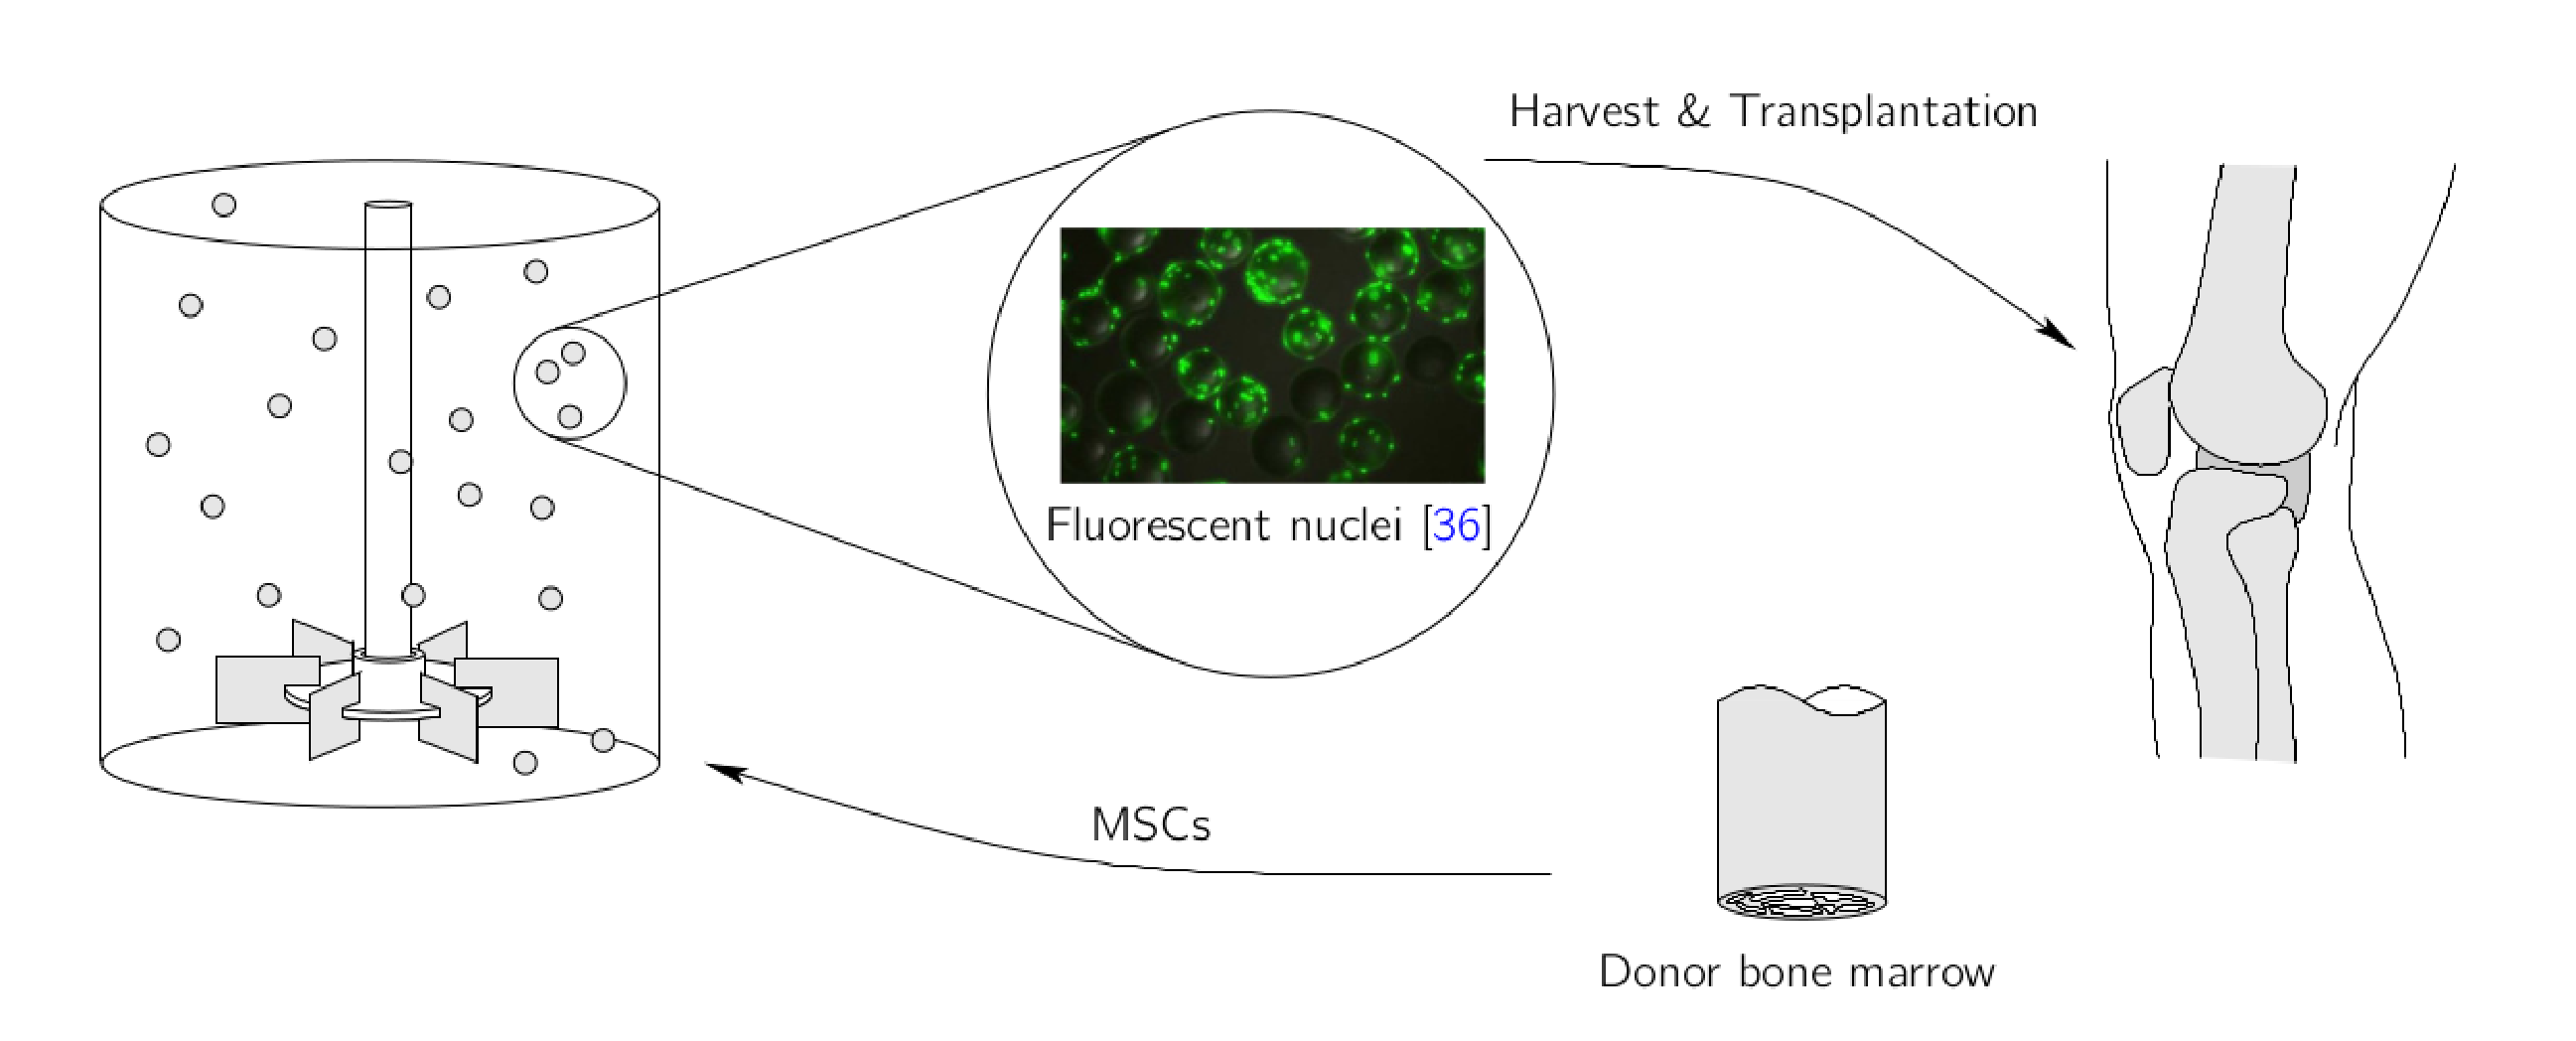
\includegraphics[width=\columnwidth]{fig/overview.eps}
  \vfill
\end{frame}

\begin{frame}[t]
\frametitle{1. Introduction -- Current challenges}
  \begin{itemize}
    \item Main flow solver already implemented in BOFFIN
    \item Adequate growth and metabolism kinetics for stem cells
    \item Simulation of rotor stator interactions
  \end{itemize}

\end{frame}

\section{Review}





\begin{frame}[t]
  
  \frametitle{Polysized nanoparticle dispersions}
  
  \vspace{-0.5\baselineskip}
  \begin{minipage}[t]{0.6\columnwidth}\vskip0pt
  \justifying\structure{Physical assumptions}
  \begin{itemize}
  \item Very many particles
  \vspace{\itemskip}
  \item Negligible particle inertia
  \vspace{\itemskip}
  \item Polydispersity with respect to size $l$
  \end{itemize}
  \end{minipage}\hfill
  \begin{minipage}[t]{0.38\columnwidth}\vskip0pt
  \resizebox{\columnwidth}{!}{\input{fig/particlesRectangle.pstex_t}}
  \end{minipage}\\
  \vspace{0.5\baselineskip}
  
  \structure{Governing equation}\\
  \justifying The evolution of a particle size distribution in space $\xbf$ and time $t$ is governed by the population balance equation (PBE) \cite{Hulburt1964}.
  \begin{equation*}
  \begin{split}
    \frac{\partial N(l, \xbf, t)}{\partial t} &+ \sum_{j = 1}^{3} \frac{\partial u_j(\xbf, t) N(l, \xbf, t)}{\partial x_j} 
    + \tcbhighmath{\frac{\partial G(l) N(l, \xbf, t)}{\partial l}} \\
    &= \sum_{j = 1}^{3} \frac{\partial}{\partial x_j}\left(D_p(\xbf, t) \frac{\partial N(\l, \xbf, t)}{\partial x_j}\right) + \dot{s}(l, N(\cdot, \xbf, t))
  \label{eq:pbe}
  \end{split}
  \end{equation*}
  
  \structure{Which discretization scheme ought to be applied along $l$?}\\
  \justifying The fields $\Hbf(\xbf, t)$ parameterizing $N(\cdot, \xbf, t)$ constitute particle phase scalars.
  \begin{equation*}
    N(\cdot, \xbf, t) \quad\longrightarrow\quad \Hbf(\xbf, t) = (H_1(\xbf, t), \ldots, H_{n_l}(\xbf, t))^T
  \end{equation*}

\end{frame}

%%%%%%%%%%%%%%%%%%%%%%%%%%%%%%%%%%%%%%%%%%%%%%%%%%%%%%%%%% FRAME %%%%%%%%%%%%%%%%%%%%%%%%%%%%%%%%%%%%%%%%%%%%%%%%%%%%%%%%%%%%%

\begin{frame}[t]
  
  \frametitle{Resolution of particle size distributions}
  
  \vspace{-\baselineskip}
  \begin{minipage}[t]{0.46\columnwidth}\vskip0pt
  \structure{Fixed $l$-grid} ($n_l \sim 500$)
  \begin{center}
  \resizebox{0.65\columnwidth}{!}{\input{fig/smallFixed.pstex_t}}
  \end{center}
  \vspace{-\baselineskip}
  {\footnotesize(Hounslow et al. 1988; Qamar et al. 2006; ...)} \nocite{Hounslow1988, Qamar2006}
  \end{minipage}\hfill
  \begin{minipage}[t]{0.46\columnwidth}\vskip0pt
  \structure{Adaptive $l$-grid} ($n_l \sim 50$)
  \begin{center}
  \resizebox{0.65\columnwidth}{!}{\input{fig/smallAdaptive.pstex_t}}
  \end{center}
  \vspace{-\baselineskip}
  {\footnotesize(Duarte and Baptista 2008; Lim et al. 2001; Sewerin and Rigopoulos 2017; ...)} \nocite{Lim2001, Duarte2008, Sewerin2017}
  \end{minipage}
  \vspace{\baselineskip}

  \structure{My objective} is to develop an economic $l$-discretization scheme that ...
  \begin{itemize}
%   \vspace{\itemskip}
%   \item resolves particle size distributions,
  \vspace{\itemskip}
  \item\justifying can be generalized to more than one particle property (while mitigating the curse of dimensionality?) and
%   \vspace{\itemskip}
%   \item employs a minimum number of scalars and
  \vspace{\itemskip}
  \item is applicable to growth-dominated populations.
  \end{itemize}
  
  \begin{snugshade}
  \justifying Can $n_l$ be reduced by preempting information about potential shapes of the particle size distribution? A reduced-order representation in $l$?
  \end{snugshade}
  
\end{frame}

%%%%%%%%%%%%%%%%%%%%%%%%%%%%%%%%%%%%%%%%%%%%%%%%%%%%%%%%%% FRAME %%%%%%%%%%%%%%%%%%%%%%%%%%%%%%%%%%%%%%%%%%%%%%%%%%%%%%%%%%%%%

\begin{frame}[t]

  \frametitle{The method of characteristics}
  
  % Reasons for considering alternative discretization schemes (other than adaptive):
  % - Is it possible to reduce the number of particle phase scalars yet further?
  % - The adaptive grid method is still subject to the curse of dimensionality! - Applicability to more than one property questionable.
    
  For brevity, we first consider the spatially homogeneous PBE for $N(l, t)$
  \begin{equation*}
    \frac{\partial N}{\partial t} + \tcbhighmath{\frac{\partial G N}{\partial l}} = \dot{s} \quad\text{on}\quad [0, L] \times [0, \infty)
  \end{equation*}

  \structure{A change in perspective}\\
  \justifying By introducing a coordinate transformation $l = \bar{l}(\tau, t)$ and defining $F(\tau, t) = N(\bar{l}(\tau, t), t)$, the PBE may be recast in terms of $F(\tau, t)$ as
  \begin{equation*}
  \begin{split}
    \frac{\partial F}{\partial t}
    + \tcbhighmath{\frac{1}{w} \frac{\partial F}{\partial\tau} 
    \left(\left.G\right|_{\bar{l}} - \frac{\partial\bar{l}}{\partial t}\right)}
    = \left.\dot{s}\right|_{\bar{l}} - \left.\frac{\partial G}{\partial l}\right|_{\bar{l}} F
  \label{eq:pbe:F}
  \end{split}
  \end{equation*}
  where $w = \partial\bar{l}/\partial\tau$. Note that the $\tau$-advection term vanishes if
  \begin{equation*}
    \frac{\partial\bar{l}}{\partial t} = \left.G\right|_{\bar{l}} \quad\Rightarrow\quad \frac{\partial F}{\partial t} =
    -\left.\frac{\partial G}{\partial l}\right|_{\bar{l}} F + \left.\dot{s}\right|_{\bar{l}}
  \label{eq:pbepod}
  \end{equation*}
%   Here, $\bar{l}(\tau, \cdot)$ defines a characteristic particle size curve.
  \justifying\structure{Particle phase scalars}\\
  ... are defined with the aid of shape functions $\phibf(\tau)$ and $\psibf(\tau)$.
  \begin{equation*}
    F(\tau, t) = \phibf(\tau)^T \abf(t), \quad
    \frac{\partial\bar{l}(\tau, t)}{\partial\tau} = \exp\left(\psibf(\tau)^T\bbf(t)\right)
  \label{eq:discrete}
  \end{equation*}

\end{frame}

%%%%%%%%%%%%%%%%%%%%%%%%%%%%%%%%%%%%%%%%%%%%%%%%%%%%%%%%%% FRAME %%%%%%%%%%%%%%%%%%%%%%%%%%%%%%%%%%%%%%%%%%%%%%%%%%%%%%%%%%%%%

\begin{frame}[t]

  \frametitle{Direct discretization}
  
  \justifying\structure{How do $\abf$ and $\bbf$ evolve in time?}\\
  The Galerkin projections of the equations governing $F(\tau, t)$ and $\bar{l}(\tau, t)$ onto the spans of $\{\phi_i\}_{i = 1}^{n_\phi}$, $\{\psi_j\}_{j = 1}^{n_\psi}$ yield \cite{Miller1981}
  \begin{align*}
    \int_{0}^{L} w \left(\frac{\partial F}{\partial t} 
    + \left.\frac{\partial G}{\partial l}\right|_{\bar{l}} F - \left.\dot{s}\right|_{\bar{l}} \right)^2 \, d\tau 
    &= \underset{\dot{\abf}}{\text{Min!}} \\
    \int_{\Lcal} \left(\frac{\partial\bar{l}}{\partial t} - \left.G\right|_{\bar{l}}\right)^2 \, d\tau 
    &= \underset{\dot{\bbf}}{\text{Min!}}
  \end{align*}
%   The length of $l$-space $[0, L]$ remains unchanged if $\bbf(t)$ obeys
  subject to the parameterizations of $(F, \bar{l})$ and the `onto'-constraint
  \begin{equation*}
    \frac{d}{dt} \bigg(\int_{0}^{L} \exp\left(\psibf(\tau)^T\bbf(t)\right) \, d\tau - L\bigg) = 0
  \end{equation*}
%   The necessary conditions for optimality yield evolution laws for $\abf(t)$, $\bbf(t)$, $\lambda(t)$.
  \structure{Interim summary}
  \begin{center}
  \resizebox{0.99\columnwidth}{!}{\input{fig/pbepodVariables.pstex_t}}
  \end{center}
  
\end{frame}

%%%%%%%%%%%%%%%%%%%%%%%%%%%%%%%%%%%%%%%%%%%%%%%%%%%%%%%%%% FRAME %%%%%%%%%%%%%%%%%%%%%%%%%%%%%%%%%%%%%%%%%%%%%%%%%%%%%%%%%%%%%

\begin{frame}[t]

  \frametitle{Necessary conditions of optimality}
  
  \structure{Spatially homogeneous evolution equations}
  \begin{align*}
    \Abf \frac{d\abf}{dt} &= \int_{0}^{L} \phibf \left.\dot{s}\right|_{\bar{l}} w \, d\tau
    - \int_{0}^{L} \left.\frac{\partial G}{\partial l}\right|_{\bar{l}} \phibf \phibf^T w \, d\tau \abf \\
    \Cbf \frac{d\bbf}{dt} &= \int_{\Lcal} \cbf \left.G\right|_{\bar{l}} \, d\tau - \lambda \left.\cbf\right|_{L}
    \quad\text{with}\quad
    \left.\cbf\right|_{L}^T \frac{d\bbf}{dt} = 0
  \end{align*}
  
  \structure{Extension to the spatially inhomogeneous case}
  \begin{align*}
    &\Abf \left\{\frac{\partial\abf}{\partial t} + u_j \frac{\partial\abf}{\partial x_j} 
    - \frac{\partial}{\partial x_j} \left(D_p \frac{\partial\abf}{\partial x_j}\right) \right\}
    = \int_{0}^{L} \phibf \left.\dot{s}\right|_{\bar{l}} w \, d\tau \\
    &\phantom{\Abf}+ \left(\Bbf - \int_{0}^{L} \left.\frac{\partial G}{\partial l}\right|_{\bar{l}} \phibf \phibf^T w \, d\tau\right) \abf
    - \left(2 D_p \int_{0}^{L} \frac{\partial\bar{l}}{\partial x_j} \phibf \frac{d\phibf^T}{d\tau} \, d\tau\right) \frac{\partial\abf}{\partial x_j} \\
    &\Cbf \left\{\frac{\partial\bbf}{\partial t} + u_j \frac{\partial\bbf}{\partial x_j} - \frac{\partial}{\partial x_j}\left(D_p \frac{\partial\bbf}{\partial x_j}\right)\right\} = 
    \Dbf + \int_{\Lcal} \cbf \left.G\right|_{\bar{l}} \, d\tau - \lambda \left.\cbf\right|_{L}
  \end{align*}
  subject to $\left.\cbf\right|_{L}^T \partial\bbf/\partial t = 0$. Here, $\cbf$ is an auxiliary $\bbf$-dependent vector and $\Abf$, $\Bbf$, $\Cbf$ and $\Dbf$ are matrices also depending on $\bbf$.

\end{frame}

%%%%%%%%%%%%%%%%%%%%%%%%%%%%%%%%%%%%%%%%%%%%%%%%%%%%%%%%%% FRAME %%%%%%%%%%%%%%%%%%%%%%%%%%%%%%%%%%%%%%%%%%%%%%%%%%%%%%%%%%%%%

\begin{frame}[t]

  \frametitle{Choosing shape functions}
  
  \vspace{-0.75\baselineskip}
  \begin{minipage}[t]{0.45\columnwidth}\vskip0pt
  \structure{Local shape functions}
  \begin{center}
  \resizebox{0.85\columnwidth}{!}{\input{fig/pbepodLocal.pstex_t}}
  \end{center}
  \justifying This leads to a characteristics-based adaptive grid method (CAGM).
  \end{minipage}\hfill
  \begin{minipage}[t]{0.45\columnwidth}\vskip0pt
  \structure{Global shape functions}
  \begin{center}
  \resizebox{0.85\columnwidth}{!}{\input{fig/pbepodGlobal.pstex_t}}
  \end{center}
  \justifying Here, representative shapes may be informed by prior observations (PBE-POD).
  \end{minipage}\\
  \vspace{\baselineskip}

  \structure{Proper orthogonal decomposition (POD)} \cite{Holmes2012}\\
  \justifying ... is a methodology based on a singular value decomposition for identifying the latent structure or hidden basis of a dataset matrix.
  \begin{itemize}
  \vspace{\itemskip}
  \item The leading POD vectors of training solutions to the PBE are chosen as $\tau$-discrete shapes $\phibf(\tau)$, $\psibf(\tau)$.
  \end{itemize}

\end{frame}

%%%%%%%%%%%%%%%%%%%%%%%%%%%%%%%%%%%%%%%%%%%%%%%%%%%%%%%%%% FRAME %%%%%%%%%%%%%%%%%%%%%%%%%%%%%%%%%%%%%%%%%%%%%%%%%%%%%%%%%%%%%

\begin{frame}[t]

  \frametitle{Calibrating shape functions}
  
  \newcommand{\snapf}{\left(\begin{array}{@{}c>{\columncolor{black!10}}cc@{}} F_1(\tau_1) &F_2(\tau_1) &\cdots \\ F_1(\tau_2) &F_2(\tau_2) &\cdots \\ \vdots &\vdots &\ddots \end{array}\right)}
  \newcommand{\snapv}{\left(\begin{array}{@{}c>{\columncolor{black!10}}cc@{}} \bar{l}_1(\tau_1) &\bar{l}_2(\tau_1) &\cdots \\ \bar{l}_1(\tau_2) &\bar{l}_2(\tau_2) &\cdots \\ \vdots &\vdots &\ddots \end{array}\right)}
  \newcommand{\vecphi}{\left(\begin{array}{@{}c>{\columncolor{black!10}}cc@{}}\phi_1(\tau_1) &\phi_2(\tau_1) &\cdots \\ \phi_1(\tau_2) &\phi_2(\tau_2) &\cdots \\ \vdots &\vdots &\ddots \end{array}\right)}
  \newcommand{\vecpsi}{\left(\begin{array}{@{}cc@{}}\psi_1(\tau_1) &\cdots \\ \psi_1(\tau_2) &\cdots \\ \vdots &\ddots \end{array}\right)}
  \resizebox{\columnwidth}{!}{\input{fig/pbepodTraining.pstex_t}}

\end{frame}

%%%%%%%%%%%%%%%%%%%%%%%%%%%%%%%%%%%%%%%%%%%%%%%%%%%%%%%%%% FRAME %%%%%%%%%%%%%%%%%%%%%%%%%%%%%%%%%%%%%%%%%%%%%%%%%%%%%%%%%%%%%

\begin{frame}[t]
  
  \frametitle{Target application}
  
  \justifying As test case, we consider the dispersion and growth of a particle population with hat-shaped inflow size distribution in a laminar plane jet.
  \vspace{-0.5\baselineskip}
  
  \begin{figure}
  \begin{center}
  \resizebox{\columnwidth}{!}{\input{fig/planejetSchematic.pstex_t}}
  \caption[Geometrical setup of a laminar plane jet test case]{Geometrical setup and inflow boundary conditions.}
  \label{fig:setup}
  \end{center}
  \end{figure}
    
\end{frame}

%%%%%%%%%%%%%%%%%%%%%%%%%%%%%%%%%%%%%%%%%%%%%%%%%%%%%%%%%% FRAME %%%%%%%%%%%%%%%%%%%%%%%%%%%%%%%%%%%%%%%%%%%%%%%%%%%%%%%%%%%%%

\begin{frame}[t]
  
  \frametitle{Training in a perfectly stirred reactor}
  
  \structure{Governing equation} with $G_0 = \SI{0.5}{nm/s}$
  \begin{equation*}
    \frac{\partial N(l, t)}{\partial t} + \frac{\partial G_0 N(l, t)}{\partial l} = 0
  \end{equation*}
  
  \structure{Training data generation}
  \begin{itemize}
  \vspace{\itemskip}
  \item CAGM with $n_{\phi} = 64$, $n_{\psi} = 53$
  \vspace{\itemskip}
  \item Solutions for $F(\tau, t)$ and $\bar{l}(\tau, t)$ sampled at \SI{1}{/s} for $t \in [0, \SI{25}{s}]$
  \vspace{\itemskip}
  \end{itemize}

  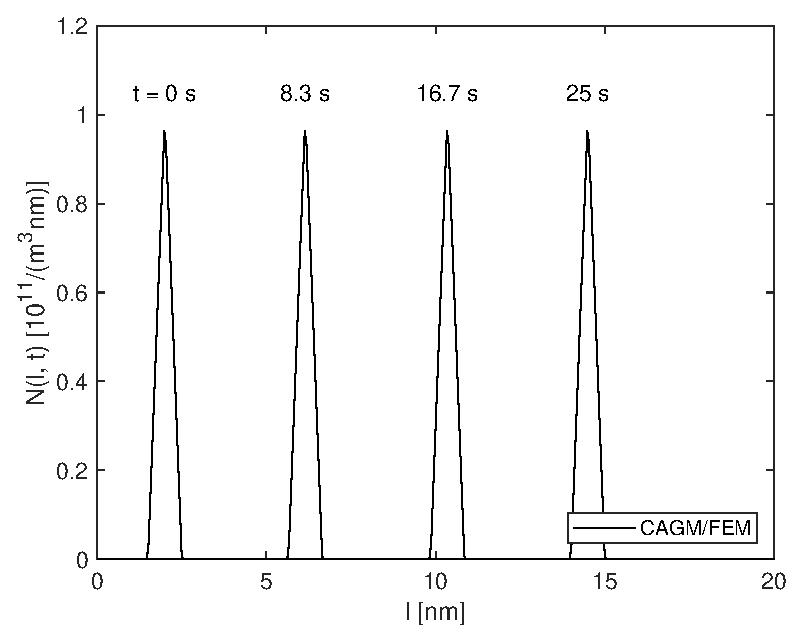
\includegraphics[height=0.38\columnwidth,clip]{fig/pbe_pod_hat.eps}\hfill
  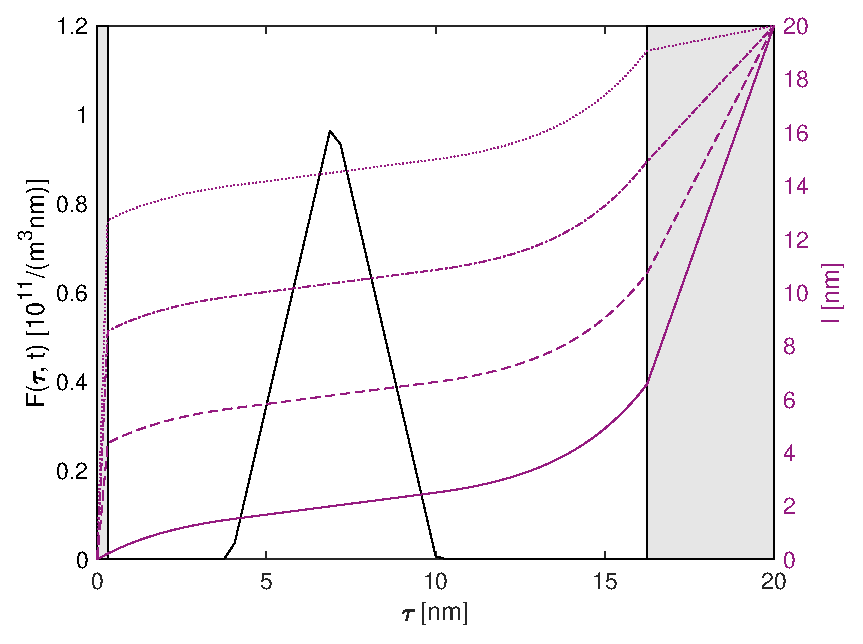
\includegraphics[height=0.38\columnwidth,clip]{fig/pbe_pod_psr_fl.eps}\\
  
\end{frame}

%%%%%%%%%%%%%%%%%%%%%%%%%%%%%%%%%%%%%%%%%%%%%%%%%%%%%%%%%% FRAME %%%%%%%%%%%%%%%%%%%%%%%%%%%%%%%%%%%%%%%%%%%%%%%%%%%%%%%%%%%%%

\begin{frame}[t]
  
  \frametitle{Training in a steady-state plug flow reactor}
  
  \structure{Governing equation} with $G_0 = \SI{0.5}{nm/s}$, $D_p = \SI{2.5e-6}{m^2/s}$
  \begin{equation*}
    U_j \frac{\partial N(l, x)}{\partial x} + G_0 \frac{\partial N(l, x)}{\partial l}
    = D_p \frac{\partial^2 N(l, x)}{\partial x^2}
  \label{eq:plugflow}
  \end{equation*}
  
  \structure{Training dataset}
  \begin{itemize}
  \vspace{\itemskip}
  \item CAGM with $n_{\phi} = 64$, $n_{\psi} = 53$
  \vspace{\itemskip}
  \item The coordinate transformation \textit{absorbs} all advective transport in $l$.
  \vspace{\itemskip}
  \end{itemize}
  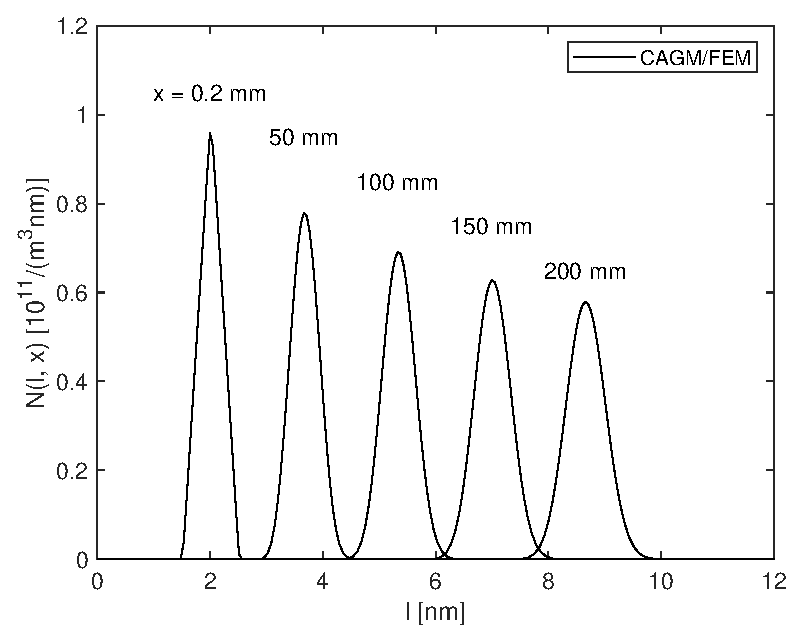
\includegraphics[height=0.38\columnwidth,clip]{fig/plugflow_N.eps}\hfill
  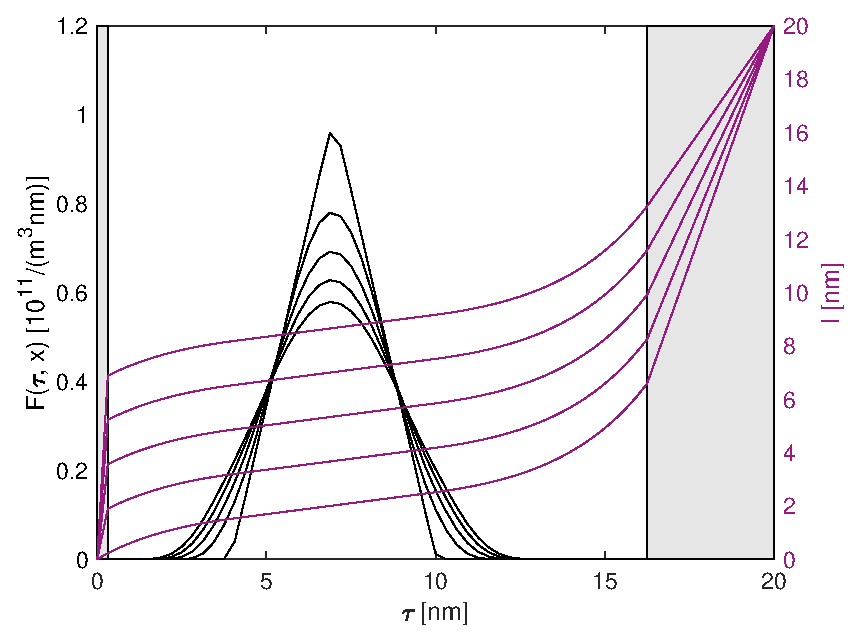
\includegraphics[height=0.38\columnwidth,clip]{fig/plugflow_Fl.eps}\\

\end{frame}

%%%%%%%%%%%%%%%%%%%%%%%%%%%%%%%%%%%%%%%%%%%%%%%%%%%%%%%%%% FRAME %%%%%%%%%%%%%%%%%%%%%%%%%%%%%%%%%%%%%%%%%%%%%%%%%%%%%%%%%%%%%

\begin{frame}[t]
  
  \frametitle{Reducibility}
  
  \justifying Since a POD eigenvalue $\lambda_k$ quantifies the energy in the dataset matrix $\Acal \in \Rset^{n \times m}$ covered by the eigenvector $\phibf_k$, we retain $n_\phi$ modes with
  \begin{equation*}
   n_\phi = \arg \min_{k} \left( 1 - \frac{\sum_{i = 1}^{k} \lambda_i}{\sum_{j = 1}^{\min(n, m)} \lambda_j} \leq \lambda_{\max} \right)
  \end{equation*}
  and similarly for $n_\psi$. Here, $\lambda_{\max}\in[0, 1)$ represents a \textit{loss threshold}.
  
  \begin{minipage}[t]{0.49\columnwidth}\vskip0pt\centering\small
  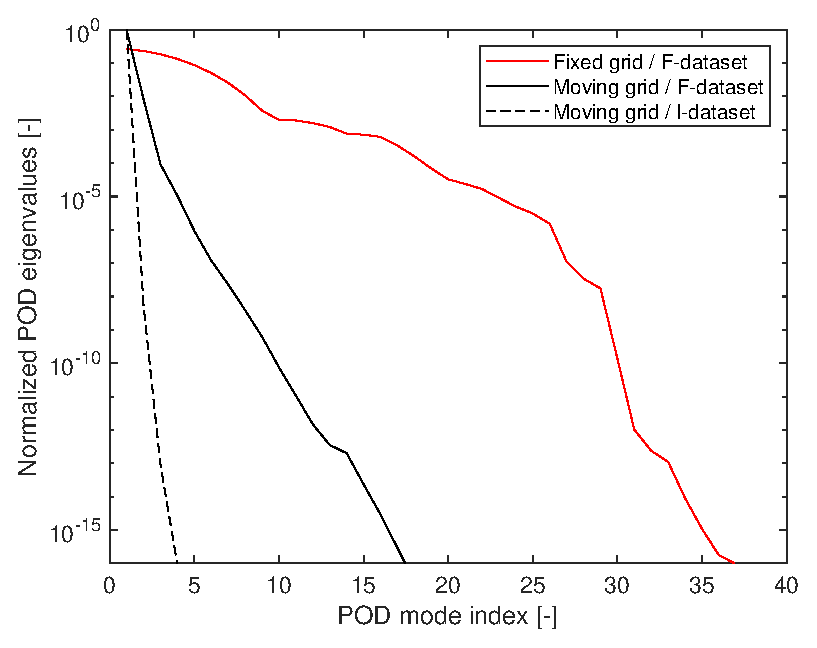
\includegraphics[height=0.75\columnwidth,clip]{fig/plugflow_decay.eps}\\
  \structure{(a)} Decay of eigenvalues.
  \end{minipage}\hfill
  \begin{minipage}[t]{0.49\columnwidth}\vskip0pt\centering\small
  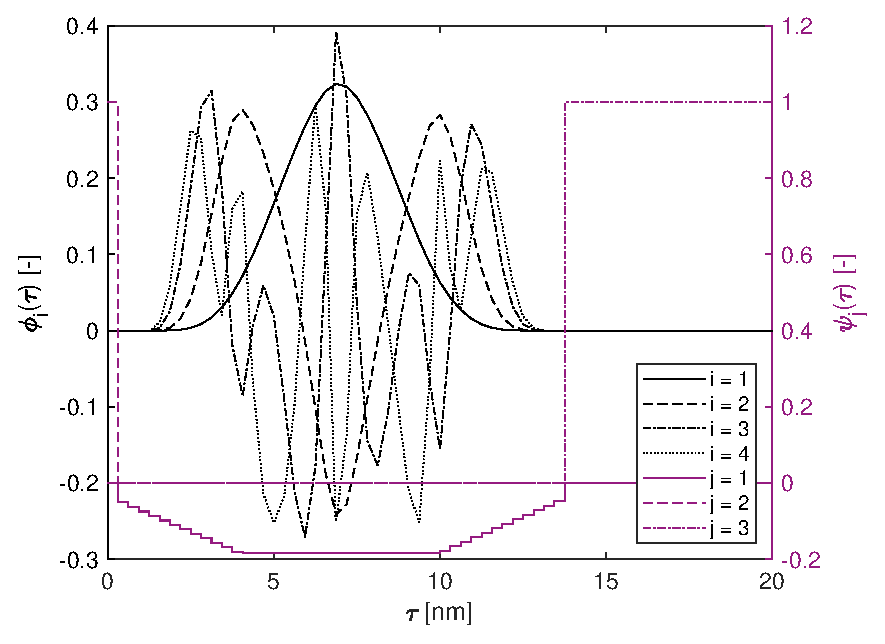
\includegraphics[height=0.75\columnwidth,clip]{fig/plugflow_II_phi.eps}\\
  \structure{(b)} Calibrated shape functions.
  \end{minipage}\\
    
  % Show trained shape functions on the left (both \phi and \psi)
  
  % Mention criteria for choosing shape functions
  
  % Show decay in POD eigenvalues on the right; include POD eigenvalues for fixed grid solution for comparison

\end{frame}

%%%%%%%%%%%%%%%%%%%%%%%%%%%%%%%%%%%%%%%%%%%%%%%%%%%%%%%%%% FRAME %%%%%%%%%%%%%%%%%%%%%%%%%%%%%%%%%%%%%%%%%%%%%%%%%%%%%%%%%%%%%

\begin{frame}[t]
  
  \frametitle{Convergence properties of the PBE-POD method}
  
  \begin{center}
  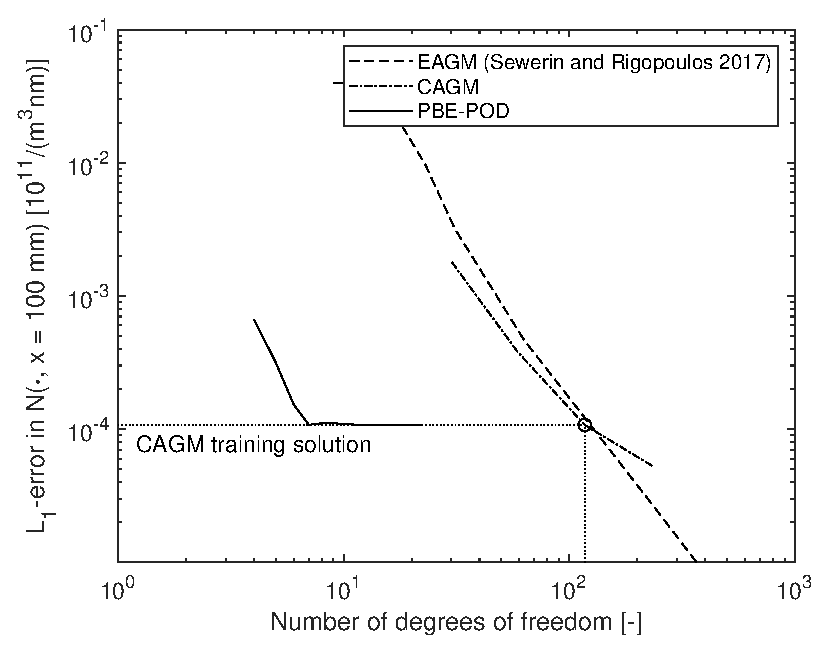
\includegraphics[width=0.65\columnwidth,clip]{fig/plugflow_convergence.eps}
  \end{center}
  
  \structure{Observations}
  \begin{itemize}
  \vspace{\itemskip}
  \item Reapplication to training problem $\longrightarrow$ Best possible accuracy
  \vspace{\itemskip}
  \item The PBE-POD method achieves a moderate accuracy of $\sim\SI{e-4}{/m}$ for an order of magnitude fewer dofs than an adaptive grid method.
%   \vspace{\itemskip}
%   \item For $n_\phi = 5$, $n_\psi = 9$, the relative PBE-POD $L_1$-error amounts to \num{7.3e-5} and is time-independent.
  \end{itemize}

\end{frame}

%%%%%%%%%%%%%%%%%%%%%%%%%%%%%%%%%%%%%%%%%%%%%%%%%%%%%%%%%% FRAME %%%%%%%%%%%%%%%%%%%%%%%%%%%%%%%%%%%%%%%%%%%%%%%%%%%%%%%%%%%%%

\begin{frame}[t]
  
  \frametitle{Plane jet test case}
  
  \vspace{-0.5\baselineskip}
  \begin{minipage}[t]{0.7\columnwidth}\vskip0pt
  \resizebox{\columnwidth}{!}{\input{fig/planejetContour.pstex_t}}\\
  \end{minipage}\hfill
  \begin{minipage}[t]{0.29\columnwidth}\vskip0pt
  \hfill\structure{Particle loading}\\
  \end{minipage}  
  
  \begin{minipage}[t]{0.36\columnwidth}\vskip0pt
  \justifying\structure{Accuracy} for $\lambda_{\max} = 10^{-5}$\\
  \begin{itemize}
  \vspace{\itemskip}
  \item Perfectly stirred\\reactor (PSR):\\$n_\phi = 1$, $n_\psi = 3$
  \vspace{\itemskip}
  \item Plug flow reactor\\(PFR):\\$n_\phi = 4$, $n_\psi = 3$
  \end{itemize}
  \end{minipage}\hfill
  \begin{minipage}[t]{0.57\columnwidth}\vskip0pt  
  \hfill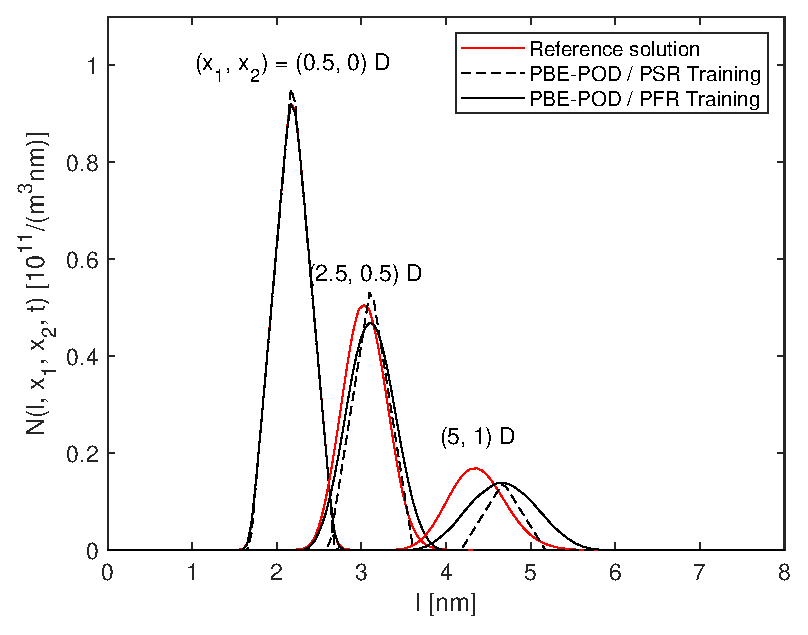
\includegraphics[width=\columnwidth,clip]{fig/planejet_psds_xr.eps}
  \end{minipage}

\end{frame}

%%%%%%%%%%%%%%%%%%%%%%%%%%%%%%%%%%%%%%%%%%%%%%%%%%%%%%%%%% FRAME %%%%%%%%%%%%%%%%%%%%%%%%%%%%%%%%%%%%%%%%%%%%%%%%%%%%%%%%%%%%%

\begin{frame}[t]
  
  \frametitle{Efficacy in parameterizing the particle size distribution}
  
  \begin{minipage}[t]{0.42\columnwidth}\vskip0pt
  \justifying\structure{Convergence properties}\\[0.25\baselineskip]
  \begin{itemize}
  \item Governing equations satisfied in least-squares sense%
  \vspace{\itemskip}
  \item Training data limitations
  \vspace{\itemskip}
  \item Shape functions acquire local features as $\lambda_{\max} \rightarrow 0$
  \end{itemize}
  \end{minipage}\hfill
  \begin{minipage}[t]{0.54\columnwidth}\vskip0pt
  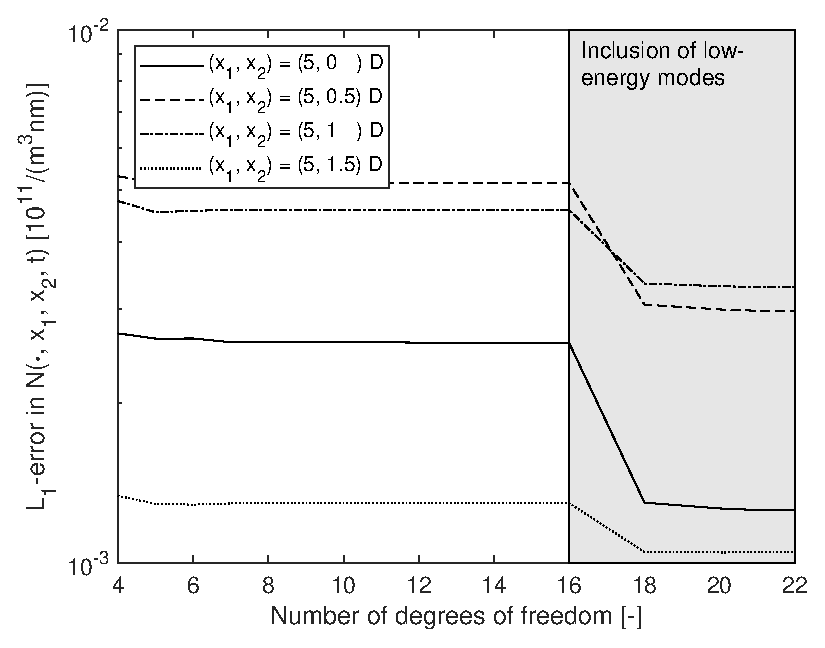
\includegraphics[width=\columnwidth,clip]{fig/planejet_convergence_l1.eps}   
  \end{minipage}\\[0.25\baselineskip]

  \justifying\structure{Runtimes}\\
  ... for degrees of freedom matched on a similar $L_1$-accuracy at $(5, 0) D$
  \begin{table}[t]\small\centering
  \begin{tabular}{l*{3}{c}}
  \toprule
    \multicolumn{1}{c}{Method}
  & \multicolumn{1}{c}{Degrees of freedom [-]}
  & \multicolumn{1}{c}{Runtime per time step [s]} \\
  \midrule
    EAGM
  & 29
  & \num{4.17e-02} \\
    CAGM
  & 27
  & \num{4.42e-02} \\
    PBE-POD
  & 7
  & \num{5.75e-02} \\
  \bottomrule
  \end{tabular}
  \end{table}

\end{frame}

%%%%%%%%%%%%%%%%%%%%%%%%%%%%%%%%%%%%%%%%%%%%%%%%%%%%%%%%%% FRAME %%%%%%%%%%%%%%%%%%%%%%%%%%%%%%%%%%%%%%%%%%%%%%%%%%%%%%%%%%%%%

\begin{frame}[t]
  
  \frametitle{Summary and outlook}
  
  \justifying By synthesizing
  \begin{enumerate}
  \vspace{\itemskip}
  \item the notion of characteristics based on an $(\xbf, t)$-dependent coordinate transformation on particle size space and
  \vspace{\itemskip}
  \item a constrained Galerkin projection with 
  \vspace{\itemskip}
  \item a POD-based training procedure
  \vspace{\itemskip}
  \end{enumerate} 
  
  we developed a direct solution method for the PBE which
  
  \begin{itemize}
  \vspace{\itemskip}
  \item tolerates growth dominated regimes,
  \vspace{\itemskip}
  \item attains a moderate accuracy in solutions for the size distribution at very few degrees of freedom.
  \end{itemize}
  \vspace{0.5\baselineskip}
  
  \structure{Open challenges}
  \begin{itemize}
  \vspace{\itemskip}
  \item Nucleation and coagulation sources?
  \vspace{\itemskip}
  \item Bivariate distributions?
  \end{itemize}
  \vspace{0.5\baselineskip}
  
  \justifying For more details: Sewerin, \textit{Chem. Eng. Sci.} 252, 117101, 2022.
  
\end{frame}

%%%%%%%%%%%%%%%%%%%%%%%%%%%%%%%%%%%%%%%%%%%%%%%%%%%%%%%%%% FRAME %%%%%%%%%%%%%%%%%%%%%%%%%%%%%%%%%%%%%%%%%%%%%%%%%%%%%%%%%%%%%

\begin{frame}[c]
  \frametitle{$ $}
  \begin{center}
    \structure{\Large Thank you for your attention}
  \end{center}
  \vspace{2\baselineskip}
  \justifying This project was funded by the Deutsche Forschungsgemeinschaft (DFG, German Research Foundation) within the scope of the Emmy Noether Program.
\end{frame}

%%%%%%%%%%%%%%%%%%%%%%%%%%%%%%%%%%%%%%%%%%%%%%%%%%%%%%%%%% FRAME %%%%%%%%%%%%%%%%%%%%%%%%%%%%%%%%%%%%%%%%%%%%%%%%%%%%%%%%%%%%%

\section{Bibliography}
\begin{frame}[t,allowframebreaks]

\nocite{Miller1981}
\frametitle{Bibliography}
\sloppy
\printbibliography[heading=none]

\end{frame}

\end{document}
